% CS 455, SP'24 Software Requirements Document template
% Software requirements template based on the template from
% https://tex.stackexchange.com/questions/42602/software-requirements-specification-with-latex
%
\documentclass[letterpaper,12pt,oneside,listof=totoc]{scrreprt}
\usepackage{listings}
\usepackage{underscore}
\usepackage{xcolor}
\definecolor{purple}{rgb}{0.5, 0, 0.5} % Adjust the RGB values as needed
\usepackage{graphicx}
\usepackage[bookmarks=true]{hyperref}
\hypersetup{
    bookmarks=false,                                % show bookmarks bar
    pdftitle={Software Requirements Specification}, % title
%    pdfauthor={Yiannis Lazarides},                  % author
%    pdfsubject={TeX and LaTeX},                     % subject of the document
%    pdfkeywords={TeX, LaTeX, graphics, images},     % list of keywords
    colorlinks=true,                                % false: boxed links; true: colored links
    linkcolor=blue,                                 % color of internal links
    citecolor=black,                                % color of links to bibliography
    filecolor=black,                                % color of file links
    urlcolor=purple,                                % color of external links
    linktoc=page                                    % only page is linked
}%
\def\myversion{1.0 }

\date{\today}
\author{} % suppress warning, do not fill this in
\begin{document}

% we don't use \maketitle because we overide the default title page here
\begin{titlepage}
\flushright
\rule{\textwidth}{5pt}\vskip1cm
\Huge{SOFTWARE REQUIREMENTS SPECIFICATION}\\
\vspace{1.5cm}
for\\
\vspace{1.5cm}
Shared Password Manager System\\                      %%% Update the title page text
\vspace{1.5cm}
\LARGE{Release 1.0\\}
\vspace{1.5cm}
\LARGE{Version \myversion approved\\}
\vspace{1.5cm}
Prepared by The Better Team\\
\vfill
\rule{\textwidth}{5pt}
\end{titlepage}

\tableofcontents
\listoffigures
\listoftables

\chapter*{Revision History}
% Update this table for each approved/baselined revision of the requirements
% Add the new content followed by a \hline

\begin{table}[ht]
\addcontentsline{lot}{table}{Revision History} % Add table to list of tables manually
\centering
\begin{tabular}{| c | p{0.25\textwidth} | p{0.50\textwidth} |}
\hline
Date & Description & Revised by \\
\hline
 &  &  \\
\hline
\end{tabular}
\end{table}




\chapter{INTRODUCTION}

\section{Purpose}
% THIS SECTION NEEDS MORE - Dakota %
This document exists to inform stakeholders of the functions and specification requirements of the Shared Password Manager Software System. The goal is to explain how the system shall hold a collection of passwords for various systems and keep track of them in a single, secure, accessible place. It also details the credentials, usernames, passwords, timestamps for the last time a password was updated, and notes for the password and system that each user is given. 

\section{Document Conventions}
This document conforms to the IEEE Standards Style Manual. Therefore, "shall," "should," "may," and typographic conventions are utilized based on the definitions by IEEE standards.
% how to read this document
% for example "conforms to IEEE Standards Style Manual"
% which defines "shall" "should" "may" and typographic conventions

\section{Acronyms}
\addcontentsline{lot}{table}{Acronym table} % Add table to list of tables manually
\begin{tabular}{| c | p{0.80\textwidth}|}
\hline
Acronym & Meaning\\
\hline
NFR & nonfunctional requirements \\
\hline
OpenBSD & Open Berkeley Software Distribution \\
\hline
SQL & Structured Query Language \\
\hline
NIST & National Institute of Standards and Technology \\
\hline
UI & User Interface \\
\hline
HTML & Hypertext Markup Language \\
\hline
PHP & Hypertext Preprocessor \\
\hline
AES & Advanced Encryption Standard \\
\hline
\end{tabular}
 \newline
% list of acronyms used in this document
% that the typical reader won't know

\section{Project Scope and Product Features}
% THIS SECTION NEEDS MORE - Andrew%
% This section will describe the features at a high level%
We propose a Shared Password Manager Application that stores password credentials. The system will use a website application environment to provide functionality for the three types of users to interact with the system: admin, regular, and view-only. 
To use the application, a user will first login to their account. The Application will then display options dependent on their privilege level. For admin users, they will have the ability to add/remove users, while regular users will have the functionality to view, add, and edit entered credentials. Additionally, View-only users will only have privilege to view credentials. The User Data will be stored securely in an SQLite database using a server. 
% high level description of what is in scope and what is
% out of scope for the software

% NOTES FROM FEEDBACK for this section^^^:
% "Only one application"
% "Don't separate front and back end here"
% INSERT FUNCTIONAL REQUIREMENTS HERE

%\section{References}

\chapter{OVERALL DESCRIPTION}

\section{Product Perspective}
This project solves the problem of managing a collection of shared credentials and accessing those credentials securely. It will also create a role-specific interface to interact with data based on the class of user (admin, regular, and view-only).

% background information about the software system
% for example - what high level problem does it solve and why

\section{Product Features}
List of product features \newline
% THIS SECTION NEEDS MORE - for Jagger %
1. Functional Features \newline
- Management system shall store credentials in a shared manner\newline
- There shall be three classes of Users: Admin, Regular, View-only \newline
- Admins shall have the ability to create, edit, and delete users \newline
- Regular users shall be able to add, edit, view, and delete credentials \newline
- View-only users shall only be able to view credentials \newline
\newline
2. Performance Features \newline
- The website shall feature a simple universal login screen for all users\newline
- After login, users shall be shown a screen displaying their credentials, see Figure \ref{UI2}.\newline
- The website shall load dynamically depending on the user type \newline
- The website shall have a button to add or edit a credential from the list\newline
- The Admin user shall have an extra button to view a user list\newline
- Users shall be able to view each of their stored credentials and their stored information, see Figure \ref{UI} \newline
- Users should be able to view a particular credential by clicking on an individual credential and viewing that credential, see Figure \ref{UI2}
- View-only users shall have the add and edit credential buttons greyed out. \newline
- If the user exits the session, they shall be required to log back in\newline
3. Aesthetic Features \newline
- The website shall present an interface that offers... reference chapter 7? \newline
- The website shall offer high affordance to features: add and edit credential\newline
- The website shall not overwhelm the users with harsh color patterns\newline
- Buttons a particular user cannot use shall be greyed out\newline
\newline
4. Complementary Features \newline
- A search bar shall allow users to search their account's list of stored credentials by name.
% search bar to filter out credentials/users
% The application will run on the CS server \newline
% a detailed list describing software features, NOT CODE
% may include example screens and reports
% may include activity or other UML diagrams
% The 

\begin{figure}
\centering
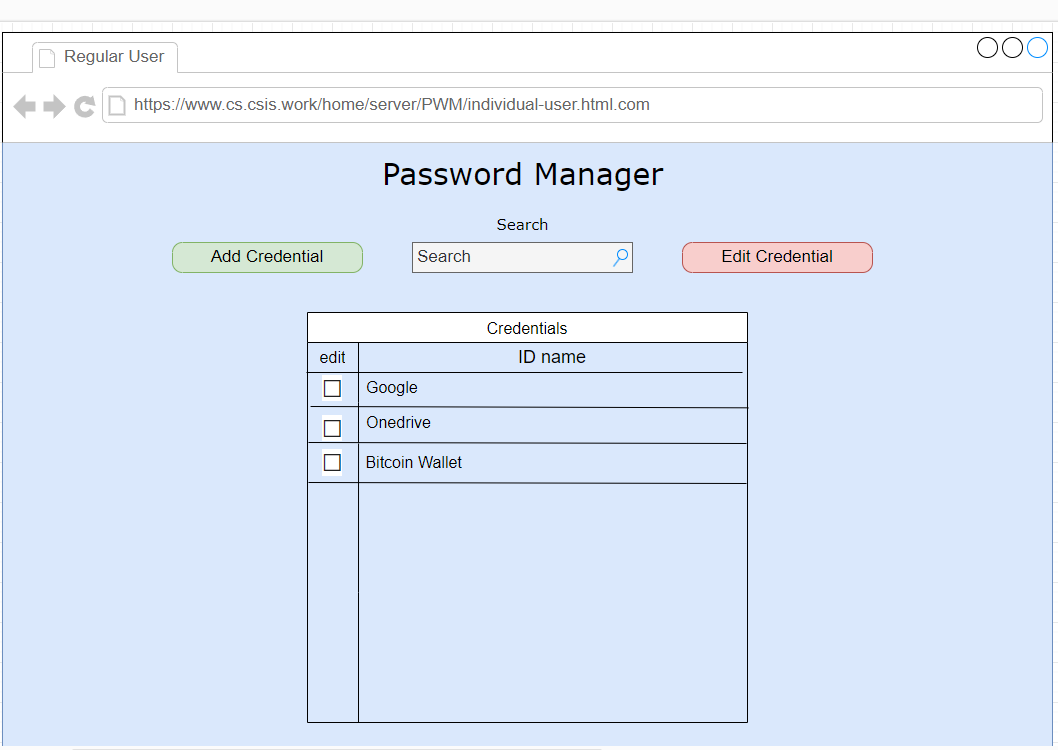
\includegraphics[width=\linewidth]{UI.png}
\caption{Regular User Diagram}
\label{UI}
\end{figure}

\begin{figure}
\centering
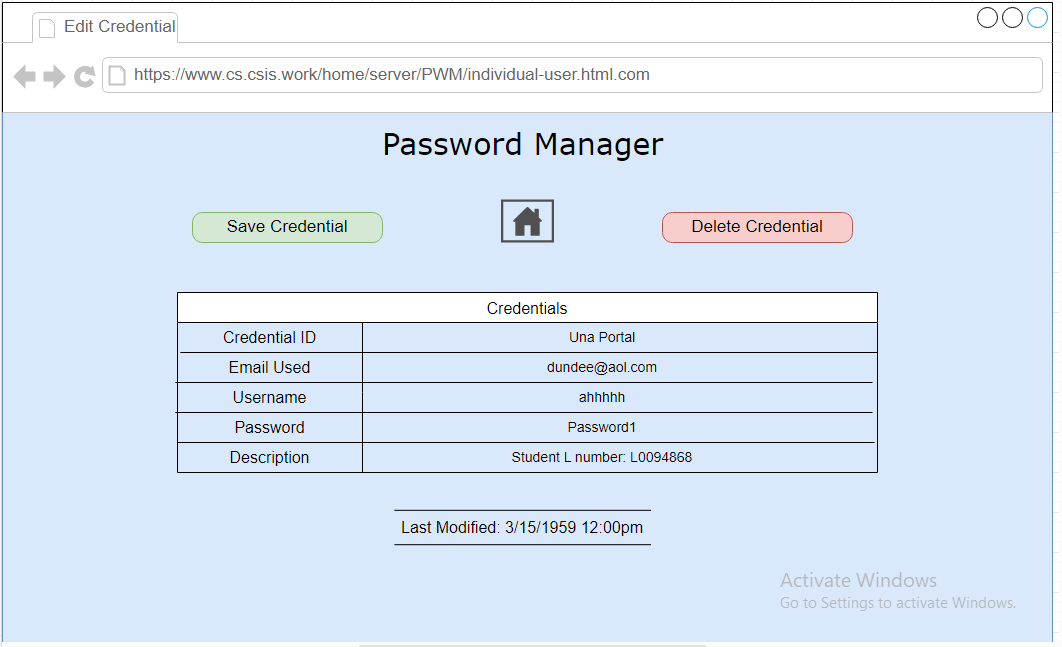
\includegraphics[width=\linewidth]{UI2.png}
\caption{View individual credential screen}
\label{UI2}
\end{figure}

\section{User Classes and Characteristics}
% THIS SECTION NEEDS MORE - Miguel%
% found some stuff about this online, characteristics is kind of broad, but includes many aspects such as the demographic of the users, their habits, needs, behaviour, etc.
% 9/24 - Miguel
There are three different classes of users interacting with the software. These three users include an admin, who can create, edit, and delete users; a regular user who can edit, view, and delete credentials; and a view-only user who can only view the credentials. A database will send and receive information to manage the storage and access of user credentials.
%Possible change? ^^
%There are four different classes of users interacting with the software. These four users include an admin, who can create, edit, and delete users; a regular user who can edit, view, and delete credentials; a view-only user who can only view the credentials; and a Database that will send and receive information from the software.

Figure~\ref{Use Case} illustrates the use case diagram that represents the different users and their interaction with the system.

\begin{figure}
\centering
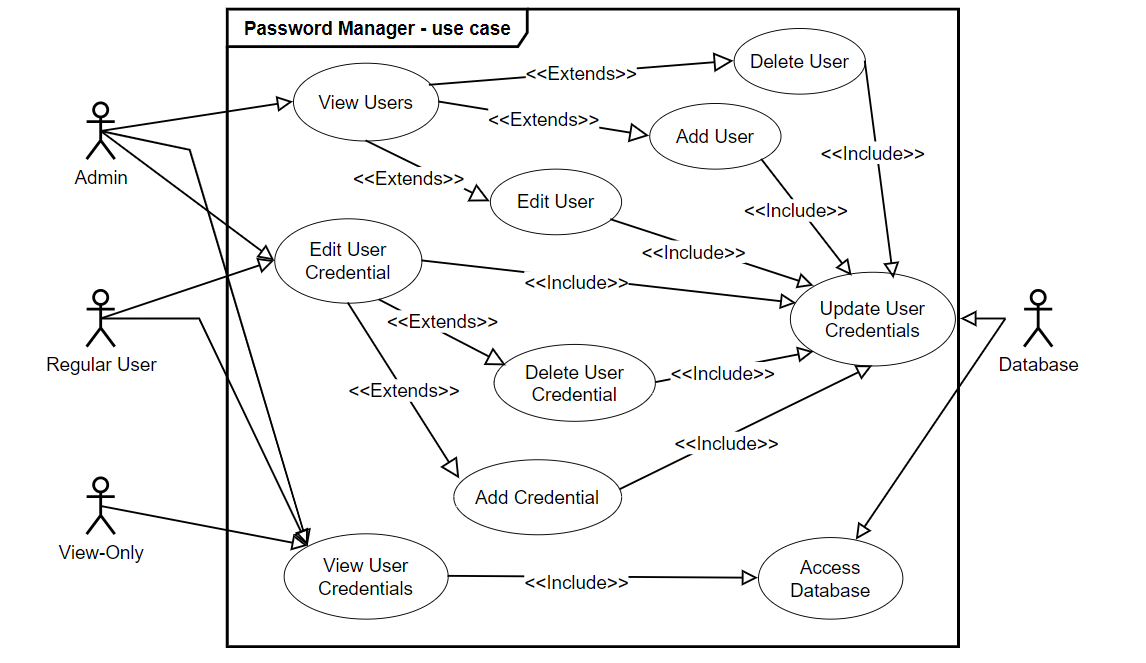
\includegraphics[width=\linewidth]{UseCaseDiagramUpdate.png}
\caption{Use Case Diagram}
\label{Use Case}
\end{figure}
% use cases and usage scenarios - NOT OOP CLASSES

\section{Operating Environment}
% THIS SECTION NEEDS MORE - %
%The software needs to be able to run on the CS server. The system will be developed in C++ and utilize the web toolkit "witty". \newline The system supports three classes of users: Admins, Regular users, and View-only users. Each user class has distinct permissions. Admin can create, edit, and delete user accounts and credentials. Regular users can view, edit, and delete shared credentials. View-only users can only view credentials.  \newline

% POSSIBLE?:
The software shall run on an OpenBSD server and shall have at least 512MB of disk space allocated. The software shall utilize a SQLite database, therefore a minimum of 512MB of RAM needs to be allocated. The server shall allocate a maximum of 2GB for storage of the data file for the SQLite database.

%The system supports three classes of users: Admins, Regular users, and View-only users. Each user class has distinct permissions. Admin can create, edit, and delete user accounts and credentials. Regular users can view, edit, and delete shared credentials. View-only users can only view credentials.  \newline


\section{Design and Implementation Constraints}
% THIS SECTION NEEDS MORE - Montana%
The finished product shall run on an OpenBSD server. The system shall be developed in the C++ language. The system shall make use of the web toolkit "witty."
% restrictions on the software system design or implementation

\chapter{NONFUNCTIONAL REQUIREMENTS}

\section{Performance Requirements}

(R1.1) The software shall support 10 users while maintaining a maximum response time of 2 seconds.\newline
(R1.2) The software shall exhibit response times of between 0-2 seconds after user input.\newline
(R1.3) Unplanned extended downtime shall not exceed 1 minute each week.\newline
(R1.4) The software shall support a minimum of two users altering credentials at the same time.\newline


\section{Safety Requirements}
This software does not require any safety requirements due to its design and intended use.

\section{Security Requirements}
(R3.1) Admin passwords shall not be obtainable by any user but that specific admin. \newline
(R3.2) Data log access shall only be available to Admin users.\newline
(R3.3) All data transfers containing user data shall be encrypted.\newline
(R3.4) Sessions shall expire after an inactivity of 30 minutes.\newline
(R3.5) The software shall enforce password authentication requirements following the NIST Digital Identity Guidelines (SP 800-63B), as specified in the Applicable Standards  (Table~\ref{tab:ApplicableStandards}). \newline
(R3.6) Accounts shall lock after three repeated failed login attempts.\newline
(R3.7) For any database login, a minimum of AES encryption shall be used before authentication.\newline
(R3.8) The software shall prevent data loss of user credentials by completing daily backups of all files to a secondary location. \newline
(R3.9) All interactions with the database shall access the database with the least privilege possible for the least amount of time.

\section{Software Quality Attributes}
(R4.1) The software shall be divided into a minimum of 2 components that can be modified individually. \newline
(R4.2) Components shall allow the ability to update without affecting other parts of the system.\newline
(R4.3) Software shall be accompanied by documentation.\newline
(R4.4) The software shall protect against unauthorized access and data breaches.\newline


\chapter{STANDARDS AND REFERENCES}

\begin{table}[h]
\centering
\caption{Applicable Standards}
\label{tab:ApplicableStandards}
\begin{tabular}{|p{5cm}|p{10cm}|}
\hline
\textbf{Standard} & \textbf{Application in Project} \\
\hline
IEEE Standard for Requirements Engineering (IEEE Std 29148-2011) & Applicable standards for this project include the IEEE Standard for Requirements Engineering (IEEE Std 29148-2011). Therefore, “shall,” “should,” “may,” and typographic conventions are utilized based on the definitions by IEEE standards. \\
\hline
NIST Digital Identity Guidelines (SP 800-63B) & Secure password standards for this project include the NIST Digital Identity Guidelines (SP 800-63B) and should enforce Single-Factor Cryptographic Software password complexity requirements for the software. Password management guidelines from NIST are utilized. \\
\hline
\end{tabular}
\end{table}
% relevant standards, NIST? ISO? IEEE?

\section{References}
[1] SQL Maestro Group, “SQLite Admin Tool - SQLite Database Browser by SQL Maestro Group,” Sqlmaestro.com, 2021. (accessed Oct. 01, 2024) \url{https://www.sqlmaestro.com/products/sqlite/maestro/help/00_04_00_system_requirements/}\newline
[2] “Basic Installation,” OpenBSD Handbook, 2024. (accessed Oct. 01, 2024). \url{https://www.openbsdhandbook.com/installation/}
[2]  NIST Password Guidelines, "NIST Special Publication 800-63-3 Digital Identity Guidelines". (accessed Oct. 01, 2024). \url{‌https://pages.nist.gov/800-63-3/sp800-63a.html}
% list any documents cited in this document

\end{document}